In this section, we propose 2 methods to solve the space optimization problem for effective meeting rooms allocation and toilet facilities usage. Our objective is to devise a solution that can efficiently use the current supply of resources. So, in our methods, we aim to find the \texttt{most optimal nearest building} and the \texttt{most optimal nearest floor} to use for booking a meeting room or using a toilet facility as per the demand and supply. 

\subsection{Method 1: Finding the most optimal nearest building}
In this method, we use spatial analysis using QGIS to predict the best nearest building for booking a meeting room or using a toilet facility. We propose an algorithm which is inspired by Song et al.\cite{song2018iterated} three-stage approach and greedy heuristics as explained in Section \ref{related_work}. 

{\setstretch{1.0}
\begin{algorithm}
  \caption{Find the most optimal nearest building}
  Inputs: Current Building \textbf{B}, Radius \textbf{R}, Objective \textbf{O}, Penalty \textbf{P}
  \begin{algorithmic}[1]
    \STATE Find all the nearest buildings within the radius R
    \STATE Calculate the \textit{weights} of these buildings: $weights = \frac{\text{Supply of the objective}}{\text{Demand of the objective}}$
    \STATE Update \textit{weights} by including correlations of the objective. 
    \STATE Calculate $probabilities = softmax(weights)$
    \STATE Penalize \textit{probabilities} to get \textit{scores} as per their physical distance from \textbf{B} and using penalty \textbf{P}.
    \STATE Optimal nearest building: $argmax(scores)$
  \end{algorithmic}
\end{algorithm}
}

The initial results of this algorithm on Current Building \textbf{B} as Alan gilbert building (Building No: 104), Radius \textbf{R} as 400m and 600m, and Objective \textbf{O} as meeting rooms are shown below.

\begin{figure}[H]
\centering
\begin{subfigure}{.5\textwidth}
  \centering
  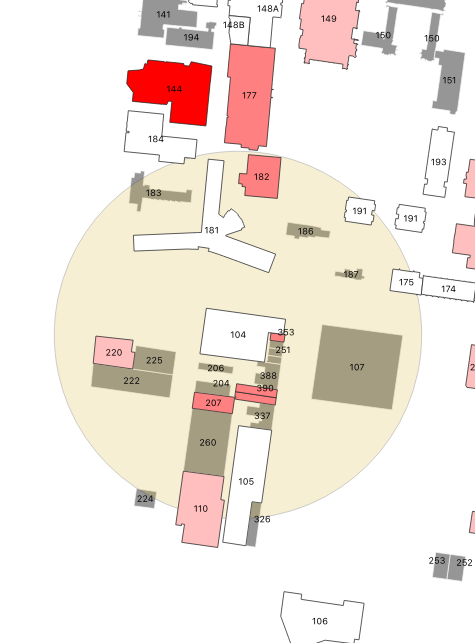
\includegraphics[width=6cm]{400m.png}
  \label{fig:400}
\end{subfigure}%
\begin{subfigure}{.5\textwidth}
  \centering
  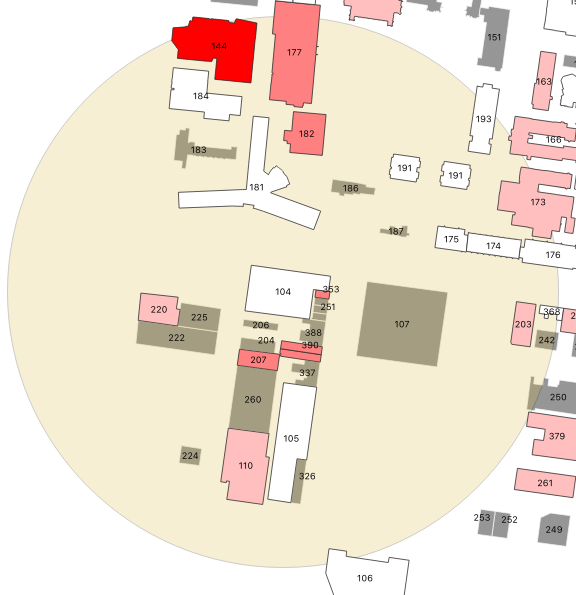
\includegraphics[width=7cm]{resources/images/600m.png}
  \label{fig:600}
\end{subfigure}
\caption{Preliminary results for Building 104 with 400m and 600m radius}
\label{fig:400-600}
\end{figure}

The concept of this algorithm is to find the most effective weights for the buildings within the provided radius. These weights are initially calculated based on the supply and demand of the objectives such as meeting rooms or toilet facility. Then, these weights are penalized on how far they are from the current building and updated based on the different correlations for the objective as discussed in Section \ref{correlations}. 

The initial results as shown in Figure \ref{fig:400-600} suggests that there is a high chance that user is not able to book a meeting room in building 104 as the weight is quite less (shown with little shade of red colour). \textbf{\textit{Currently, these weights and probabilities are not getting updated as per step 3 and 5 of the algorithm.}} So, based entirely on the supply-demand weighting scheme, algorithm running with 400m radius will suggest \texttt{building 207 (MDHS)} and 600m radius will suggest \texttt{building 144 (Kenneth Myer)} as the most optimal nearest buildings.

\subsection{Method 2: Finding the most optimal nearest floor for a building}
In this method, we have used \texttt{python} to create a model based on the greedy heuristics which can predict the most optimal nearest floor for booking a meeting room or using a toilet facility. 

{\setstretch{1.0}
\begin{algorithm}
  \caption{Find the most optimal nearest floor}
  Inputs: Current Building \textbf{B}, Current Floor \textbf{F}, Objective \textbf{O}, Penalty \textbf{P}
  \begin{algorithmic}[1]
    \STATE Get all the floors in the provided current building
    \STATE Calculate \textit{props} for supply on each floor: $props = \frac{\text{Supply of the objective at each level}}{\text{Total Supply of the objective in building}}$
    \STATE Calculate \textit{props} for demand on each floor: $props = \frac{\text{Demand of the objective at each level}}{\text{Total Demand of the objective in building}}$
    \STATE Calculate \textit{weights} for each floor: $weights = \frac{\text{Supply of the objective}\:\times\:\text{\textit{props} for supply}}{\text{Demand of the objective}\:\times\:\text{\textit{props} for demand}}$
    \STATE Update \textit{weights} by including correlations of the objective. 
    \STATE Calculate $probabilities = softmax(weights)$
    \STATE Penalize \textit{probabilities} to get \textit{scores} as per their physical distance from \textbf{F} and using penalty \textbf{P}.
    \STATE Optimal nearest floor: $argmax(scores)$
  \end{algorithmic}
\end{algorithm}
}
The model predictions using above algorithm for Current Building \textbf{B} as Kwong lee dow building (Building 263), Current Floor \textbf{F} where the user is located as Level 3, Objective \textbf{O} as meeting rooms and Penalty \textbf{P} as 0.005 is shown below.

\begin{figure}[H]
\centering
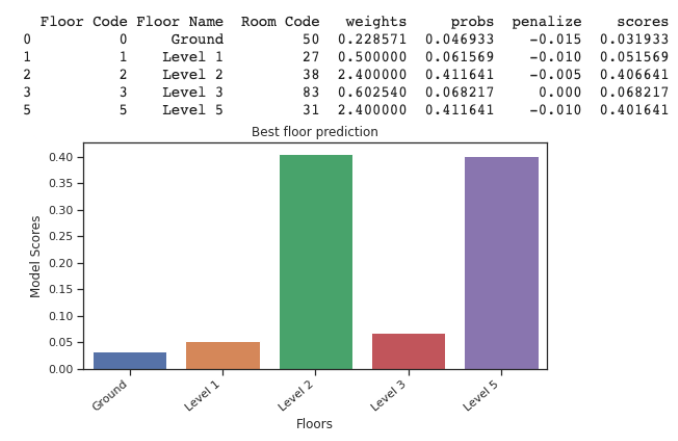
\includegraphics[width=8cm,keepaspectratio=true]{B-263}
\caption{Model scores prediction for Building 263}
\label{fig:B-263}
\end{figure}

Using the above predictions, we can say that \texttt{Level 2} will be the most optimal nearest floor for booking a meeting room after considering supply-demand weighting scheme. These results are still not considering \textbf{Step 5} of the algorithm which will further enhance the accuracy of the scores. Similarly, we can do model predictions for Current Building \textbf{B} as Redmond barry building (Building 115), Current Floor \textbf{F} where user is located as Level 1, Objective \textbf{O} as toilet facilities and Penalty \textbf{P} as 0.005. The results are shown below.

\begin{figure}[H]
\centering
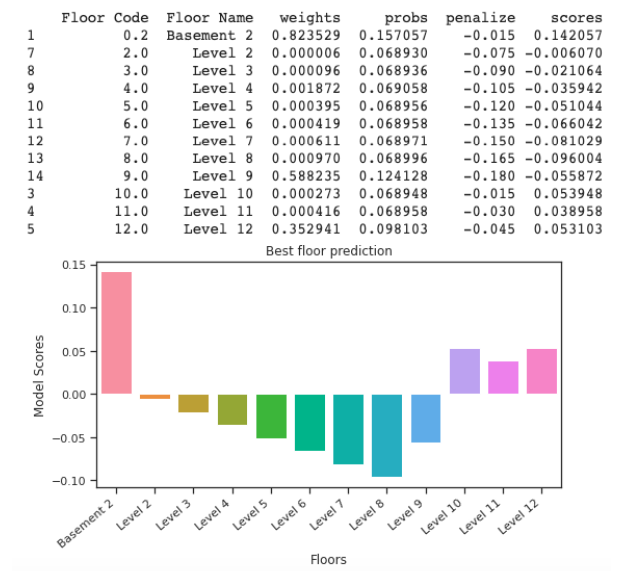
\includegraphics[width=8cm,keepaspectratio=true]{B-115}
\caption{Model scores prediction for Building 115}
\label{fig:B-115}
\end{figure}

Using the above predictions, we can say that \texttt{Basement 2} will be the most optimal nearest floor for using a toilet facility, considering all the supply-demand constraints. Again, these results are still not considering \textbf{Step 5} of the algorithm which will be implemented in the next phase of the project. 

